\section{Terahertz measurement} % TODO
% TODO describe what follows in this section

\subsection{Short review of the terahertz technology}
The electromagnetic waves in the terahertz range, roughly between 100 GHz and 10 THz, have found relatively small application in science and technology in the 20th century, compared to the development in the microwave ($<$ 100 GHz) and near-infrared ($>$ 100 THz) or optical ranges. The reason can be traced down both to the limited choice and high cost of suitable terahertz sources and detectors, and to their small efficiency and sensitivity, respectively. 

The following paragraphs show why thermal sources are not applicable to the THz range, and briefly list the most prominent sources of THz radiation that are used in research or technology. A brief overview of THz technology follows. There is a great number of literature that covers this topic in depth \cite[pp. 155-158]{lee2008book}, % TODO add
and it is also covered by theses from our group (\cite[pp. 2-30]{pashkin2004phd}, \cite[pp. 19-25]{nemec2006}, \cite[pp. 7-26]{fekete2008phd}, \cite[pp. 11-21]{sibik2010dp}, \cite[pp. 31-45]{yahiaoui2011phd}, \cite[pp. 33-38]{mics2012phd}, \cite[pp. 25-33]{skoromets2013phd}, etc.).

\paragraph{Thermal emission in the THz range}
The blackbody radiation is governed by the Planck law % TODO cite
\begin{equation}I(f, T) = \frac{2 h}{\pi^2 c^2}\frac{f^3}{e^{\frac{\h f}{kT}}-1} \mathrm{\,W\,sr^{-1}\,Hz^{-1}\,m^{-2}}, \label{eq_planck}\end{equation}
%$$ ,$$ TODO
from which follows that the luminosity in the terahertz range is always very small: Integrating over frequencies from 300 GHz to 3 THz, one obtains roughly 0.6 W sr$^{-1}$ m$^{-2}$ at the room temperature.  Furthermore, all Planck oscillators in the THz range are already fully saturated:
%  although the thermal energy at room temperature $T$ is significantly higher than the photon energy $hf$ at 1 THz
$$k_B T \approx 1.38\cdot 10^{-26} \text{ J K}^{-1} \cdot 300 \text{ K~} \approx 25.8 \text{ meV } \gg h f \approx 4.13 \text{ meV}), $$
and therefore the power radiated in the THz range can not be significantly improved by increasing the blackbody temperature. Particularly, it can be shown that in this part of the spectrum the luminosity scales only linearly with the temperature $T$; whereas the total power scales as $T^{4}$ (Stefan-Bolzmann law). Sources other than thermal have to be used.


\add{
\paragraph{Coherent continuous THz sources}
Whenever a beam of electrons (or possibly other charged particles) is subject to fast-enough acceleration at the picosecond scale, electromagnetic waves in the terahertz band are radiated. This is the case of magnetic deflection in particle accelerators, or the periodically-poled magnet, \textit{wiggler}, in the free electron laser. 
Typically, such approach finds practical application in rather large-scale facilities. 

Gyrotron
Backward wave oscillators (carcinotron)
		M-type, the most powerful, (M-BWO) and the O-type (O-BWO). The O-type delivers typically power in the range of 1 mW at 1000 GHz to 50 mW at 200 GHz. 
Free electron lasers and synchrotrons
klystron.


THz lasers
p-Ge laser
Quantum cascade lasers

Tunable THz-wave parametric generation
Optical rectification CW
Quasi-Phase- Matching Crystals (Fanned-out PPLN)


\paragraph{Pulsed THz sources}
Optical rectification
pulsed/cont

Biased and unbiased photoconductive switches
pulsed/cont

Tilted Optical Pulses in Lithium
Niobate

\paragraph{Other THz sources}

Coherent THz Radiation from Superconductors
Cerenkov-like emission of THz radiation

Terahertz radiation from shocked materials

\paragraph{Terahertz detectors}
1.3.1 Photoconductive receiving antennas . . . . . . .
1.3.2 Electrooptic sampling . . . . . . . . . . . . . . .
1.3.3 Magnetooptic sampling . . . . . . . . . . . . . .
1.3.4 Terahertz-induced lensing . . . . . . . . . . . .
1.3.5 Bolometers

}

\subsection{Terahertz time-domain spectroscopy}
The numerical data could be in some cases corroborated by experimental measurement using the \textit{time-domain terahertz spectroscopy} (TDTS) in our laboratory. 
The approach is similar to that used in the FDTD simulations. A short, broadband pulse impinges the sample, one part of its energy is transmitted, another reflected and the rest is absorbed in the sample. The transmitted pulse is then recorded by the time-domain sampling setup. The resulting transmission is computed by means of Fourier transform as a complex spectrum, which is to be normalized by the spectrum of the incident pulse.
% TODO 

\subsection{Terahertz generation and detection setup}%{{{
\begin{figure} \caption{img/exp\_THz\_sampling.pdf}  \centering 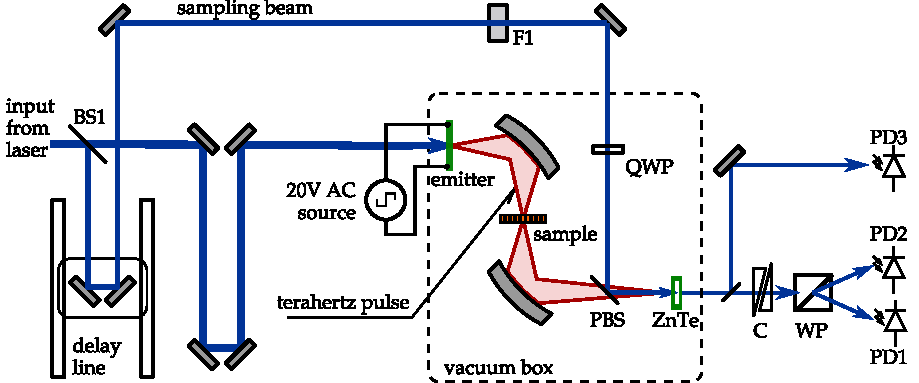
\includegraphics[width=10cm]{img/exp_THz_sampling.pdf} \end{figure} \clearpage

%The experimental geometry is somewhat similar to that used for FDTD simulations above. Also the results are similar: we get the complex amplitude transmission spectrum,  
\begin{figure}[ht] \caption{\textit{Experimental setup for terahertz time-domain spectroscopy}} \label{fg_exp} \centering 
	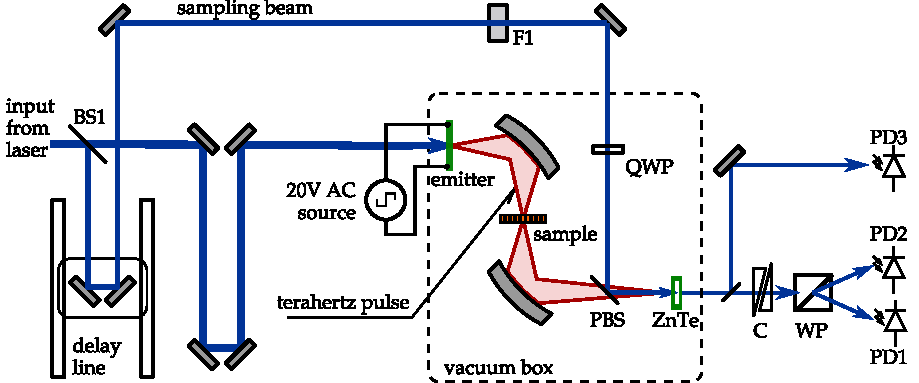
\includegraphics[width=12cm]{img/exp_THz_sampling.pdf}
\end{figure}

% TODO laser equipment
The crucial component of the TDTS generation and detection setup is the source of ultrashort optical pulses. We used \textit{Coherent Mira} femtosecond oscillator with mean power of 0.5 W, central wavelength 810 nm, and a pulse duration under 70 fs. The optical pulses were split at beamsplitter (BS1) into the \textit{probe} branch and the \textit{sampling} branch. 
\begin{itemize}
 \item{The probe branch passed through a mechanical chopper, % TODO WRONG
which is needed for synchronous detection, and impinged a terahertz emitter. The emitter, a biased interdigitated antenna on a fast-switching semiconductor, responds to an optical pulse by fast discharging and emitting of a broadband electromagnetic pulse with spectral components from 100 GHz to 3 THz. This pulse, denoted by red area to indicate its diffractive nature, passes through the sample under study followed by a pellicle beamsplitter (PBS) and finally impinges a ZnTe nonlinear crystal. } 
 \item{The \textit{sampling} branch reflects from a pair of mirrors on a delay line, acquiring a precisely controlled relative delay against the first branch. Then it is properly attenuated at filter (F1) and its polarisation is converted from linear to a circular one on a quarter-wave plate (QWP). The pellicle beamsplitter directs the optical beam along the axis of the terahertz beam.} 
\end{itemize}
%% TODO add references to other papers and theses from our group - one can not describe everything from Gouy shift to PKGraph ...
%}}}
\subsection{Scheme for simultaneous measurement of reflection and transmission}%{{{
It is theoretically possible to measure the \textit{reflection spectrum} using TDTS in a similar way the transmission spectrum was measured. However, due to the complexity of such a setup and sensitivity to sample displacement, we did not use a second sampling branch for reflected signal. Instead of using two sampling schemes, it is possible to recover the amplitude and phase reflectivity of a sample by stacking it between a pair of thick (3 and 6 mm) sapphire slabs. Thanks to the relatively high refractive index of sapphire ($N \approx 3.4$), these slabs introduce several distinct  echoes into the transmission signal.

\begin{figure} \caption{A broadband pulse passes through a single layer of microspheres randomly arranged between two sapphire slabs and is sampled by electrooptical detection.}  \centering 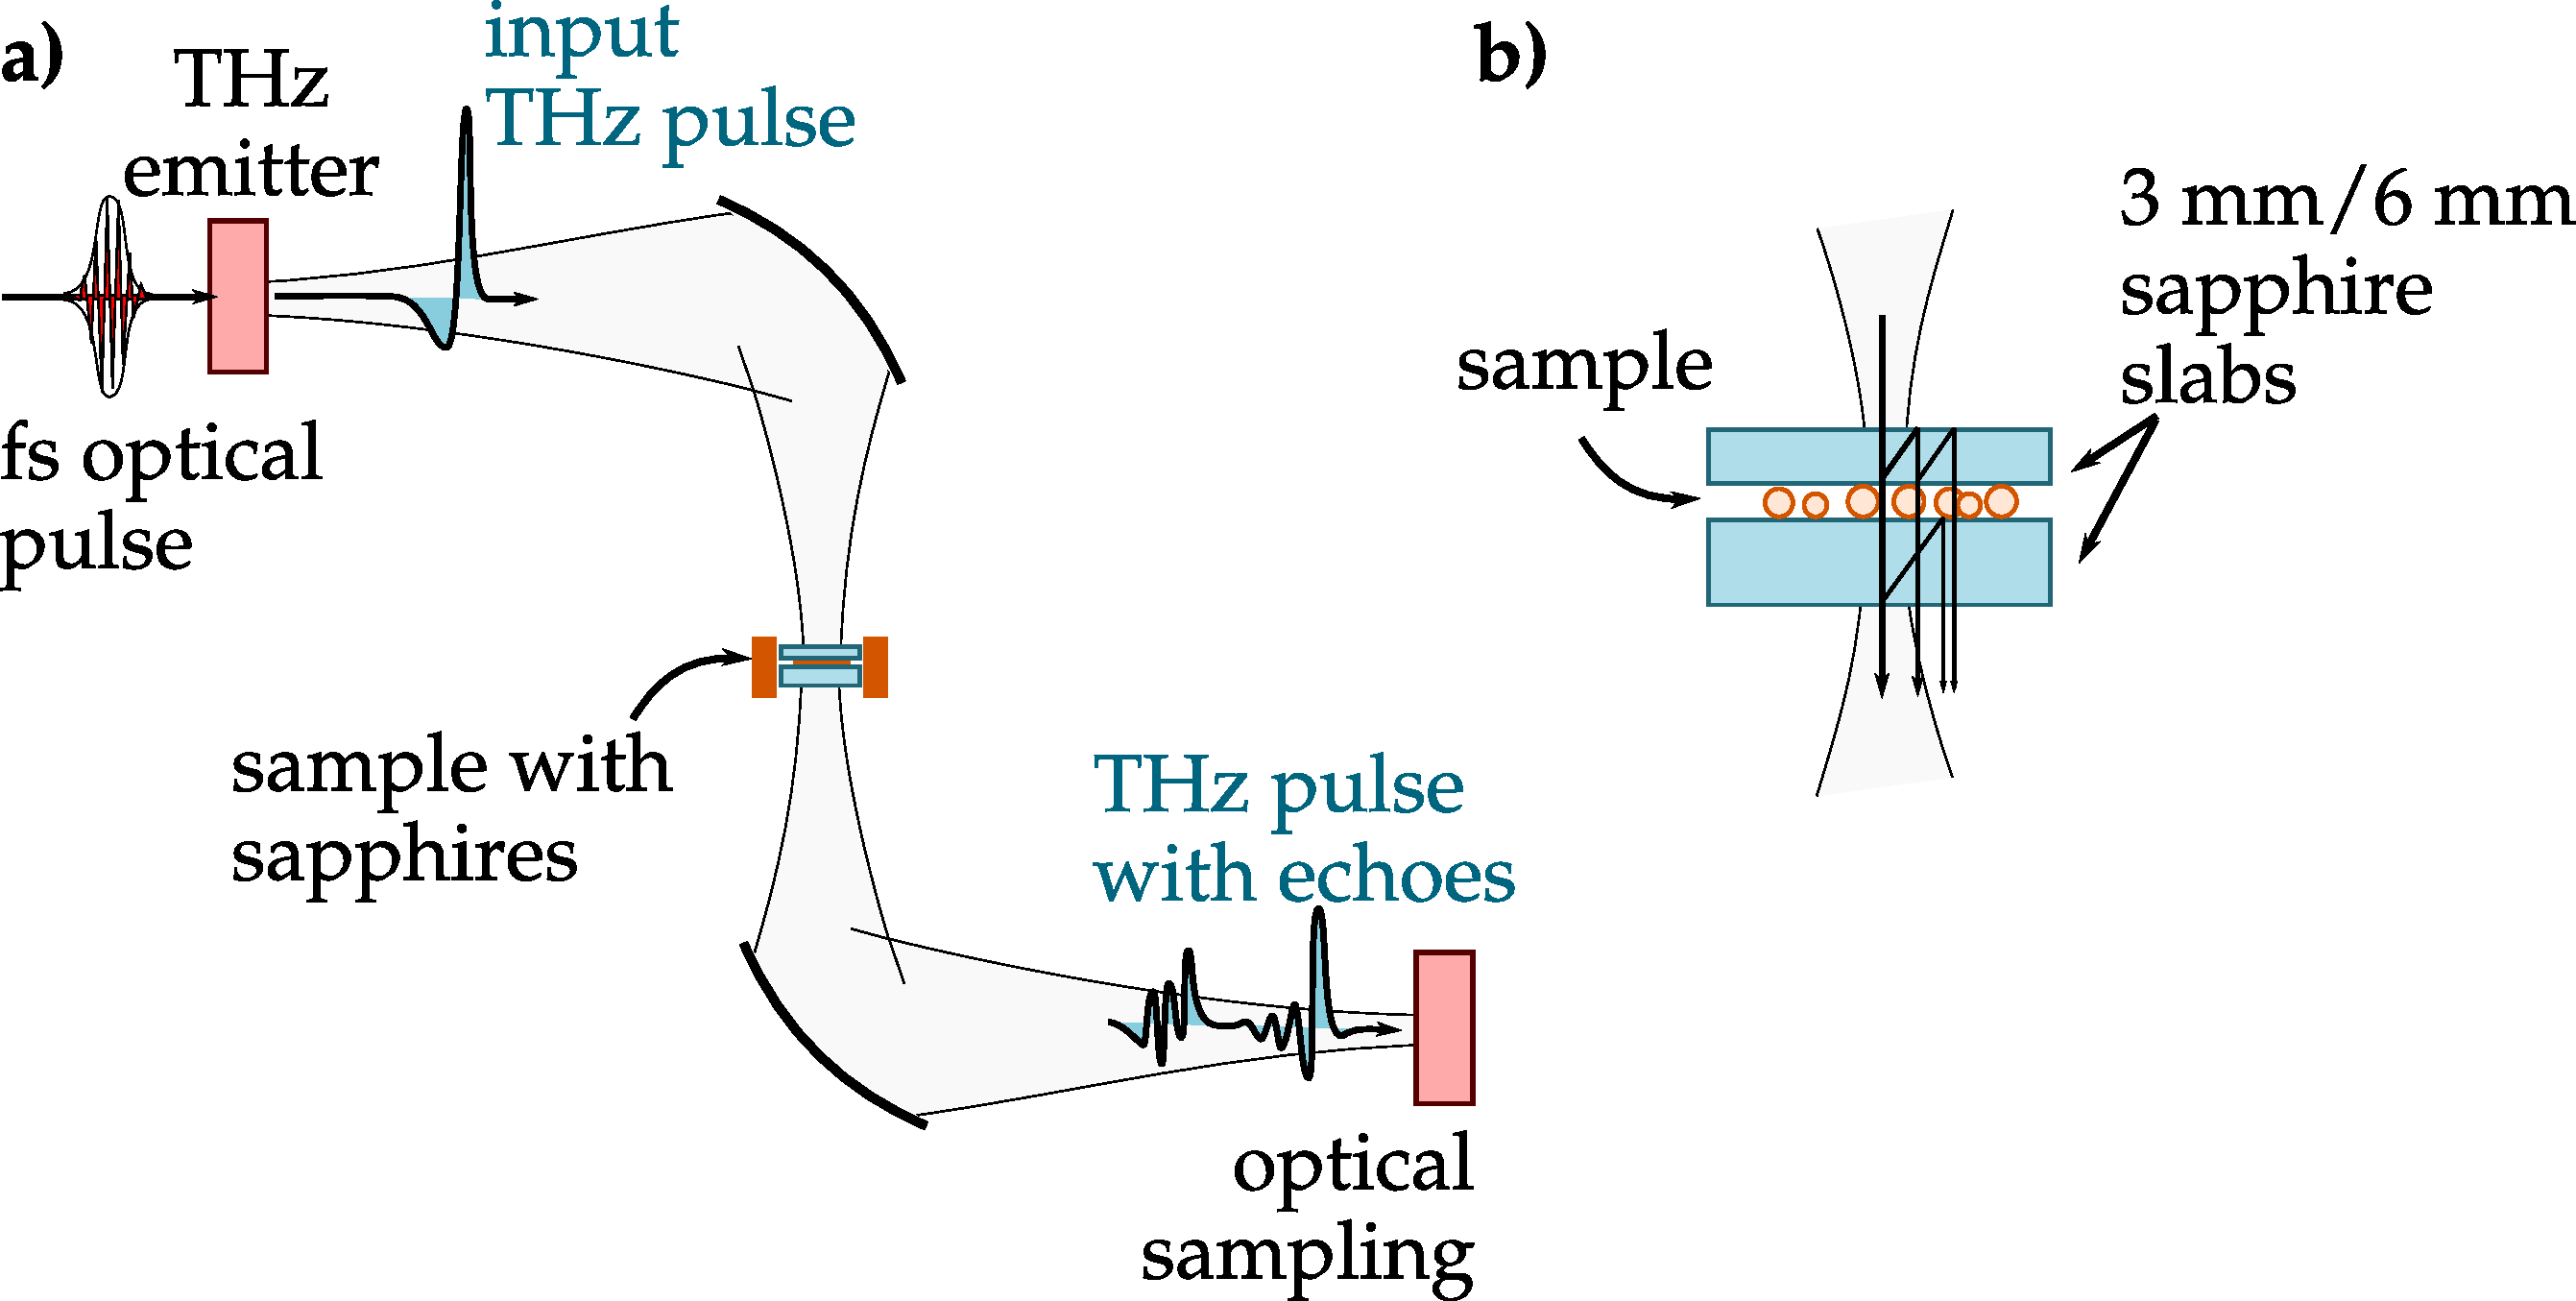
\includegraphics[width=12cm]{img/expe/sample_sapphires.pdf} \end{figure} \clearpage

If the beam divergence is neglected, each optical element can be characterised by its complex transfer function in the resulting spectrum. One needs to define three transmission functions for the beam passing the volume of the thin sapphire $A(f)$, thick sapphire $B(f)$ and of the sample $t(f)$, and two reflection functions for the beam reflected on sapphire-air interface $r_{A}(f)$ and on the sapphire-sample interface $r_S(f)$. 

The recorded overall signal has to be split into its first part  % TODO

%defines the temporal separation between the main pulse and the first echo.  The reflection and transmission of the sample can be simply reconstructed using numerical deconvolution. The results of this method were, unfortunately, less than ideal. Among the reasons may be the possible asymmetry of the studied layer between the slabs, beam divergence and very low signal of both transmission and particularly reflection in the stop-bands of the sample.

The propagation delay through $2\times 3$ mm of sapphire is roughly 70 ps, which defines the spectral resolution to 14 GHz. All spectral features in the sample transmission must be significantly broader than this value. Otherwise they not only could not be resolved, but most importantly, their ringdown would overlap in the time domain with the following echo, producing spurious results. Using a thicker sapphire could improve spectral resolution of this method, however it conflicts with the requirement for the beam being narrower than the sample \cite{nemec2009tunable} and, independently, of reducing the error caused by beam diffraction as noted in the following paragraph.

In the experiment, we observed substantial deviation  % TODO add some experimental data and  and reference them here
from the numerically predicted results, which were moreover sensitive to subtle changes in the parameters. We propose  several explanations for the experimental errors:
\begin{enumerate}
\item{The geometrical beam divergence can not be fully compensated by the transfer functions [$A(f)$, $B(f)$] of separate sapphire slabs. The deconvolution algorithm can amplify or attenuate different frequency components to compensate for the  longitudinal focus displacement of the first echo compared the focus of the first pulse. However, due to the hyperbolic shape of the gaussian beam with Rayleigh length $z_{R}$ similar to the sapphire thickness\footnote{As an approximate example, for the main frequency component $f = 1.5$ THz with wavelength $\lambda = c / f \approx 200$ $\upmu$m, for $\vartheta \lesssim 0.15$ rad as an estimated divergence of the beam from its axis, the Rayleigh half-length of a gaussian beam would be $z_{R} = \frac{\lambda}{\pi \vartheta^{2}} \gtrsim 2.8$ mm, i.e. roughly the thickness of the thinner sapphire.}, the overall effect of two sapphires can not be linearly predicted from two separate measurements of each of them.} 
 \item{The possible asymmetry of the sample with regards to the beam axis can substantially bias the measured reflectivity. This happened during the characterisation of the dielectric spheres, when the sapphire distance was defined by a $\approx$60$\upmu$m teflon spacer. The nonuniform size of the resonators required to attach them to one of the sapphire windows, which resulted in that their average and sub-average size fraction had strongly asymmetric position. } 
 \item{The sapphire slabs can influence the near field of resonances in some samples. This error should not manifest in transversally homogeneous samples (i.e. slabs), nor in samples that are made of dielectrics with much higher permittivity than that of sapphire. However for some samples such as metamaterial fishnets or other metallic resonators, the simulations confirm that resonant frequencies can be substantially altered by the vicinity of a dielectric. }
 \item{Finally, it follows from Eq. (\ref{}) % TODO reference the slab-index-retrieval procedure
 that the reliable reflection data can only be retrieved at frequencies where also the transmission amplitude is strong enough for the signal not to be dominated by noise. }
 \end{enumerate}
%}}}
\section{Sample preparation} 
\subsection{Preparation of dielectric and bars}
In the following section, the properties of periodic dielectric rods are discussed. 
A similar sample used in experiment consisted of bars from strontium titanate (SrTiO$_{3}$) with  rectangular cross-section (see Fig. \ref{fg_ebars_exp}). These bars were fabricated by femtosecond laser micro-machining from a thin slab of the dielectric \cite{yahiaoui2011tunable}.
% TODO
\subsection{Fabrication and sieving of dielectric sphere samples}
Compared to the dielectric bars, the fabrication of the dielectric spheres can be extremely simplified by the \textit{spray-drying process}. In contrast with the expensive and time-consuming \textit{top-down} processes such as laser machining, litography or polishing, this is a typical \textit{bottom-up} process, where the particles are formed all within one procedure, though certain postprocessing is needed. The following technique in a collaborating laboratory in France %% Todo reference to Patrick's group somehow
provided us with high-permittivity TiO$_{2}$ spheres with the sizes from 30 to 100 $\upmu$m. 

\begin{figure}[ht] \caption{Microphotograph of the TiO$_{2}$ spheres after preliminary sieving} \label{fg_microphoto} \centering 
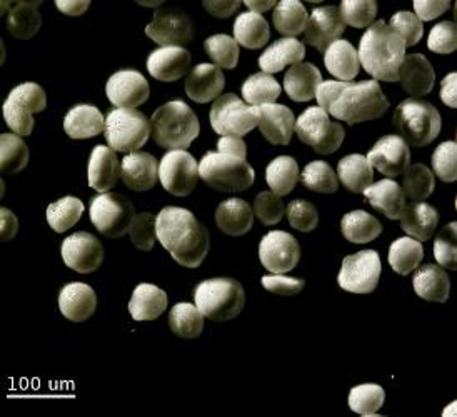
\includegraphics[height=5cm]{img/microscope_TiO2_particles.pdf}
\end{figure}

\paragraph{Spray-dry process}%{{{
Rutile (TiO$_{2}$) was ground to a powder of sub-microscopic particles. 
A suspension of these nanoparticles in ethanol was sprayed into flame. The average size of particles was determined by the solid concentration in the suspension, by feed rate and by gas flow.It immediately formed spherical droplets, which dried up and sintered in the hot air.  

The resulting particles were annealed in a furnace to further solidify. By the temperature of the furnace, the degree of recrystallization could be controlled: from microscopic grains (at around 1200  $^{\circ}$C) to a sphere consisting of few crystalline domains, which were apparent in electron microscope (annealed at\footnote{From personal communication with Dr. Patrick Mounaix} 1300--1400 $^{\circ}$C). Note the temperatures used are still far below the melting temperature of rutile (i.e. 1800 $^{\circ}$C).

Only the low-temperature annealed samples were measured by the terahertz spectroscopy in this thesis. The fine-grained rutile was assumed to be well approximated by an isotropic dielectric. The size of the constituent crystalline grains was estimated from the observation of one microsphere ground on a glass of a pollarisation microscope: unlike polycrystalline aggregates, single rutile monocrystals manifest as coloured particles due to their inherent birefringence. Therefore, the size of crystalline grains were determined in the order of few micrometers.

Similar TiO$_{2}$ microspheres are also available commercially (e.g. from Brace, GmbH), and to the author's knowledge, they are made with a similar process.
%}}}
\paragraph{Microsphere pre-sieving and other treatment}%{{{
The annealed spheres required further processing, as described by {Dr.} U-Chan Chung: 
\textit{
(\ldots) As the spheres have been sintered at high temperature, they have been separated from a platinum plate with a small soft paintbrush followed by a light milling with a agathe mortar. The goal was to separate the spheres that are welded to their neighbours due to the sintering step. All the spheres were treated in ultrasound-bath using ethanol as liquid phase. After natural drying, the sieving was performed. (\ldots) square (or rectangular) holes sieves were used. The meshes used were 106, 100, 53, 50, 40 and 38 micrometer. As a dry sieving step was performed, the particles were light milled again in order to try to break possible agglomerates which would not go through the mesh. This process was repeated 2-3 times and a final wet sieving with ethanol was performed in order to "wash" the spheres. No special measures were taken according to their shapes. (\ldots) } 
% TODO
%}}}
\paragraph{Theory of anisotropic sieves}%{{{
Triple sieving on commercial sieves in Bordeaux, weaved from stainless steel wire, did not provide narrow enough size distribution. We therefore developed detailed methods of sample refinement and characterisation. 

\begin{figure}[h] \caption{\textbf{a)} \textbf{b)} } \label{fg_sieve_pass_notpass} \centering 
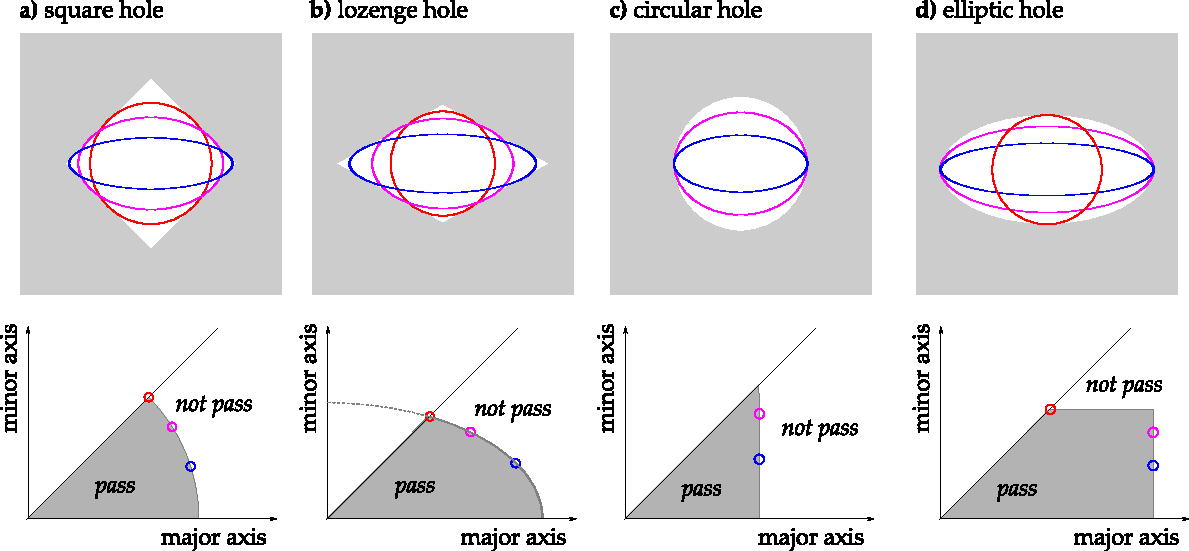
\includegraphics[width=\textwidth]{img/technology/sieve_pass_notpass.pdf}
\end{figure}
In the following, we approximated the dielectric particles by ellipsoids with three (generally different) half-axes $$r_a \leq r_b \leq r_c.$$ For the purpose of sieving, only the values of the shortest two axes, $r_a$ and $r_b$, decide whether the particle can pass through the sieve. The longest ellipsoid axis $r_c$ does not affect this, although it may influence the sieving speed. Therefore we can represent each 3-D particle with its projection on the smallest possible ellipse, which is described by its \textit{minor axis} $\equiv 2r_a$, and by its \textit{major axis} $\equiv 2r_b$. For a given shape of a hole in a homogeneous flat sieve, it is easy to determine which values of minor and major axes allow a particle to pass through, and which not. For a square sieve such area in the parameter space forms a disk around the center of origin (Fig. \ref{fg_sieve_pass_notpass}a). It can be shown that when the sieve is diagonally stretched, forming a lozenge hole shape, the area of spheres allowed to pass changes into an ellipse (Fig. \ref{fg_sieve_pass_notpass}b). When the hole shape is circular or elliptical, it is obvious that the area forms a part of a square or of a rectangle, respectively  (Fig. \ref{fg_sieve_pass_notpass}c,d).

The resonance frequency of a dielectric resonator depends on all three half-axes, $r_a \leq r_b \leq r_c$. In order to select as narrow size fraction as possible, one has to use double sieving: the above sieve not allowing the fraction of particles too big, the bottom sieve removing the fraction of particles too small. This is where the anisotropic hole shapes become useful -- the bottom sieve can exclude also all oblong particles with the difference of $r_a \leq r_b$ too big. This effect is illustrated in Fig. \ref{fg_double_sieving}, which also presents a comparison of using more usual sieves of square/lozenge holes with the effect of a couple of sieves of micromachined square/elliptic holes. Obviously, the latter approach better discriminates for the \textit{shape} of the ellipsoid. This advantage further gains on importance when the anisotropy of the sieve is low.
\begin{figure}[ht] \caption{\textbf{a)} \textbf{b)} } \label{fg_double_sieving} \centering 
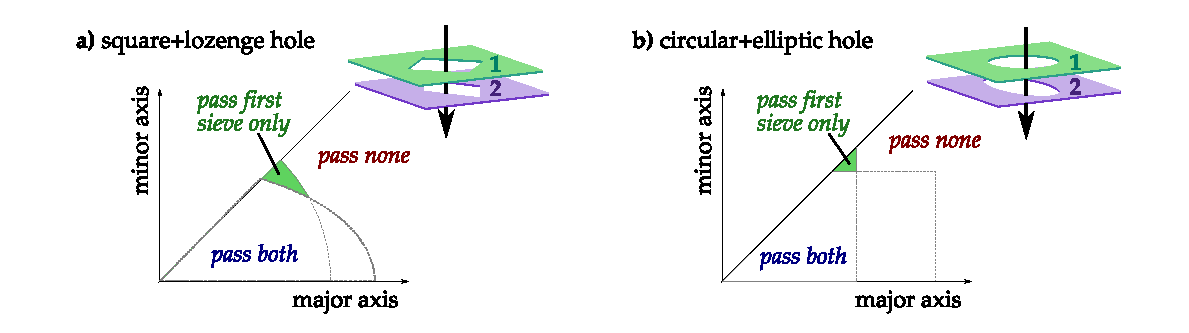
\includegraphics[width=\textwidth]{img/technology/sieve_double_sieving_fractions.pdf}
\end{figure}

% TODO 4x hole-sphere sketch  --->  maj-min binary funciton of (not)passing
It shall be noted that although we plotted a binary (\textit{pass}/\textit{not pass}) function in Figs. \ref{fg_sieve_pass_notpass} and \ref{fg_double_sieving}, the sieving speed greatly differs for different sizes of particles. This is due to lower probability of a particle passing, if its parameters are near the edge of possible-passing function. 
%For any finite sieving time, this obviously affects the statistics of particles passing the sieve, favoring the average size to be lower for short sieving times. The particles that are close to 
However, this particular fraction of particles is exactly what one is interested in during the high-accuracy sieving! The process must therefore run for long enough time, in the order of days, and with as high sieving speed as possible.
%}}}
\paragraph{First sieving apparatus}%{{{
 %Finally, they were carefully sieved in many iterations, to select a size fraction as narrow as possible.
Employing the idea of anisotropic sieves from Fig. \ref{fg_double_sieving}a, we assembled the first prototype based on nylon sieves, as depicted in Fig. \ref{fg_sieving1}. Two glass containers were lathed of a 
% diam
glass tube, and on their bottom, nylon sieves were glued. The side of the sieve holes was 60$\pm$5 $\upmu$m, and while the above sieve was kept isotropic, the bottom one was stretched by ca. 20-25 \% in diagonal direction. The nylon mesh was woven, so the threads easily bent aside, allowing oversized particles either to pass or to get stuck permanently, blocking the sieve within few minutes. To resolve the latter problem, two additional narrow glass rings were cut, with much coarser sieves glued on the bottom, to allow little spherical springs bounce beneath the sieves and to loosen the particles that got stuck in the holes. A cover on top prevented the particles to jump out of the above container. Whole stack was carefully lowered into a test tube with a greater diameter, and vibrated by a tiny electric motor glued on the bottom.
\begin{figure} \caption{\textbf{a)}\textbf{b)}\textbf{c)} TODO input of unsorted microspheres}  \centering 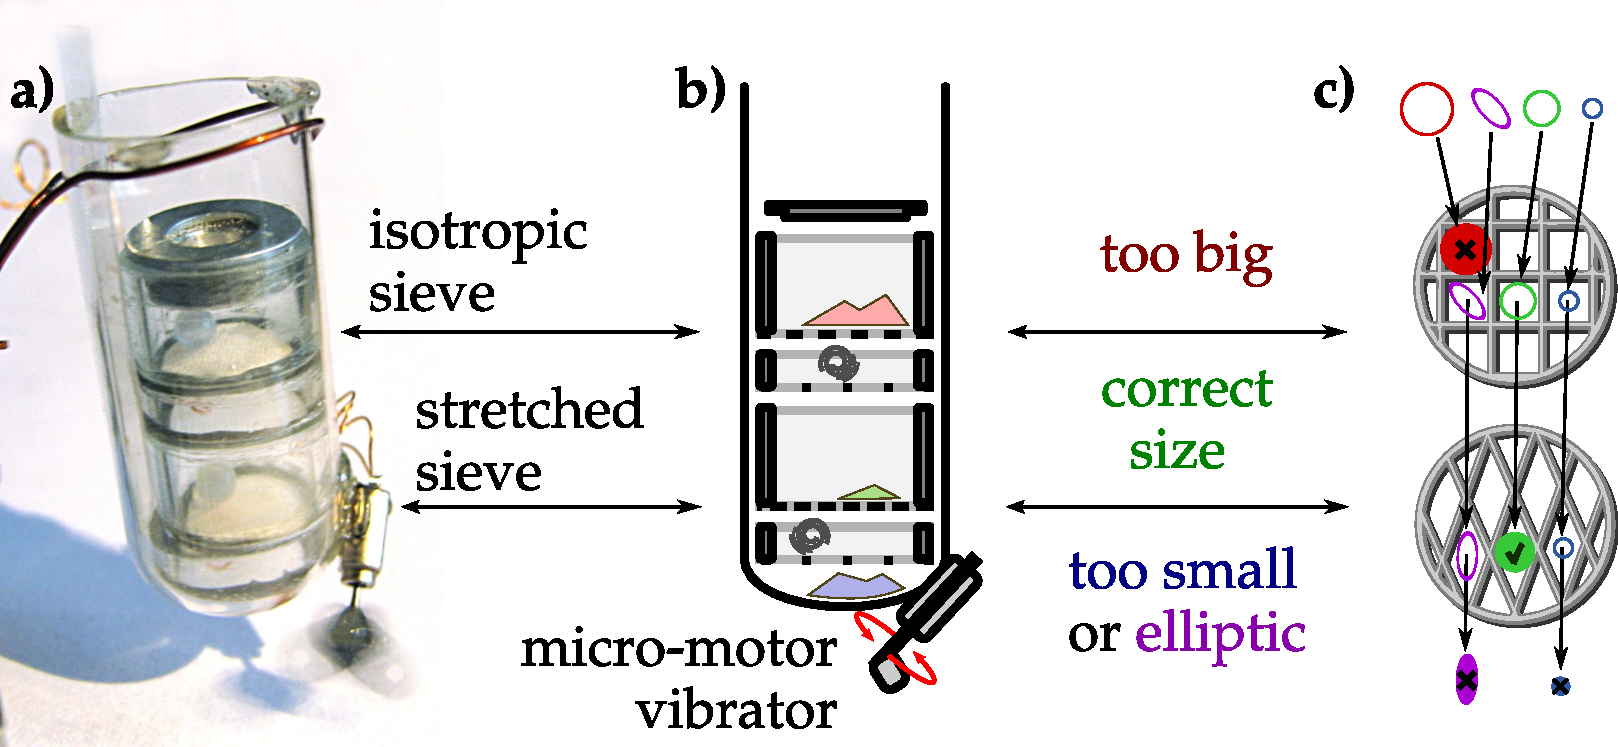
\includegraphics[width=12cm]{img/expe/sieving1.pdf} \label{fg_sieving1} \end{figure} 
%}}}
\paragraph{Second sieving apparatus}%{{{
\begin{figure}[ht] \caption{\textbf{a)} A sketch of the acoustic sieving device, and \textbf{b)} a photograph thereof} \label{fg_sieving2} \centering 
\textbf{a)}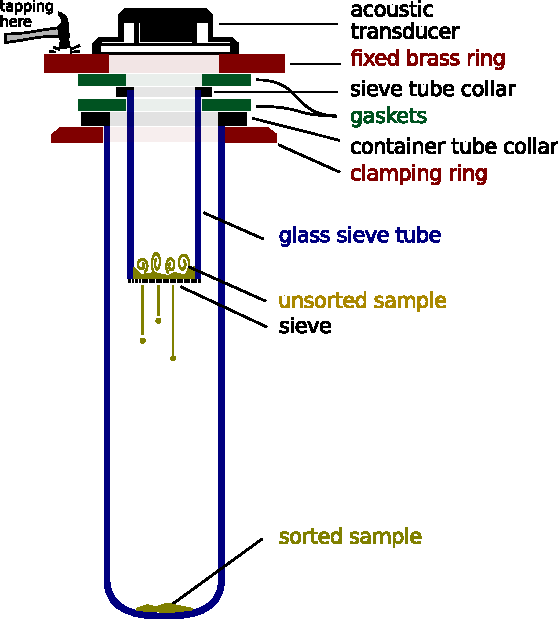
\includegraphics[height=8cm]{img/technology/sieve2_sieving_scheme.pdf}
\textbf{b)}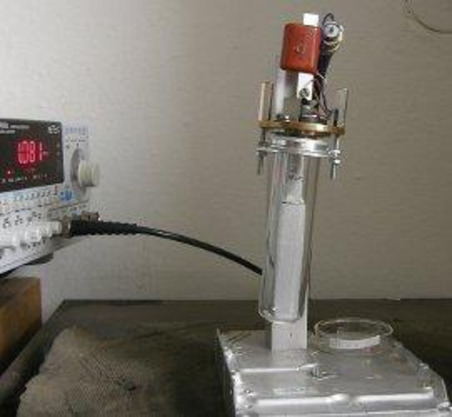
\includegraphics[height=8cm]{img/technology/sieving_m.pdf}
\end{figure}
The partially promising results and, more importantly, obvious deficiencies of the previous apparatus motivated building a second one depicted in Fig. \ref{fg_sieving2}.
Different from any other sieving apparatus known to the author, this one made use of intense vertical acoustic wave for the movement of particles. It consisted of two coaxial glass tubes: The inner tube, with outer diameter of 13 mm, had a round metallic sieve glued to its bottom, and on its upper end it was covered by a 20 mm acoustic transducer. The outer tube (90 mm long, outer diameter 26 mm) surrounded the inner one and had a round bottom, where the particles collected. 
The gaskets ensured that whole apparatus was tightly closed, preventing both sieved particles and sound from escaping. The brass ring with the transducer was fixed to a massive aluminum stand, and the rest of the structure was clamped to it by two M3 screws with nuts that allowed for easy disassembly. 

The key advantages of this novel approach are the following:
\begin{enumerate}
 \item{\textbf{The speed of sieving} is roughly proportional to the frequency at which the particles hit the sieve. The acoustic frequency of 1 kHz is rouhly two orders of magnitude higher than in usual commercialy available devices. The spheres are moreover continuously stirred, so it is ensured that a layer of over-sized particles does not occupy the sieve.} 
 \item{The upward air pressure \textbf{pulls out particles that got stuck in the sieve} in every period of acoustic vibration. This resolves the major issue of the previous prototype.} 
 \item{\textbf{Avoiding macroscopic vibrating parts}, except the membrane of a small acoustic transducer, allows the device to operate over multiple days without the risk of mechanical failure of any part.}
 \end{enumerate}


The outer tube acted as an acoustic resonator, greatly enhancing the effect of the sound when tuned to resonance around 750-900 Hz. These frequencies obviously correspond to the fundamental acoustic resonance, as the quarter-wavelength is the range from 91 to 110 mm. 

%TODO The power of the sinewave feeding the device was limited by the parameters of the acoustic transducer
A practical deficiency of this setup was that the upper opening of the transducer radiated relatively intense sound during operation. We resolved this potential issue by covering whole apparatus by a robust glass bell jar.

With the acoustic power and frequency correctly adjusted, the particles formed a cloud 5--10 mm high. One difficulty arose from that the small particles tend to attach to the surface of glass or metal, probably due to electrostatic charges on their surface. While at an average particle radius $\rho = 50$ $\upmu$m this effect was rather marginal and transient, it took only few seconds of sieving for $\rho = 20$ $\upmu$m particles to immobilize permanently on any surface. It has however proven efficient to tap the upper brass ring, as the vibration released most spheres, effectively renewing the sieving process. To ensure unattended sieving for a timespan in order of days, we added a little motorized hammer with a timing circuit. % todo add photo of the hammer

The amount of particles in one batch was limited to ca. 10--20 mm$^{3}$, otherwise the sieve would be covered with a layer too thick, which could not be efficiently lifted by the acoustic pressure.
It could however be remedied by tilting the apparatus. With a tilt of 5--10 degrees, the bulk of particles then accumulated near one side, leaving most of the sieve surface free for sieving the moving fraction of particles. According to the small amount of particles required for the terahertz spectroscopy measurements, it is however advisable to sort a batch in order of 1--3 mm$^{3}$.
%}}}
\subsection{Automatic determination of microparticle statistics}
\begin{figure}[ht] \caption{\textbf{a)} A section of a microphotograph of sample before sieving, \textbf{b)} the corresponding identification of particles in ImageJ} \label{fg_sievingstats} \centering 
\textbf{a)}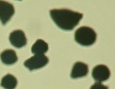
\includegraphics[height=5cm]{img/technology/imagej_photo.pdf}
\textbf{b)}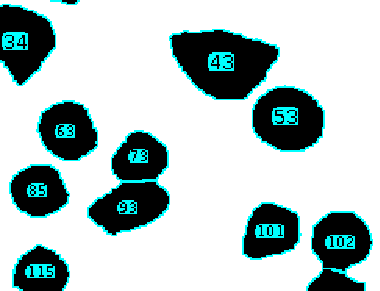
\includegraphics[height=5cm]{img/technology/imagej_found.pdf}
\end{figure}

We developed a numerical method to measure the histogram of size distribution of the particles based on a calibrated microphotograph of the sample such as in Fig. \ref{fg_sievingstats}a. This enabled to assess the sieving precision and also to predict the realistic signal by simulation.
\add{ TODO}
% TODO  add the 4-fold png figure from web

\subsection{Laser micro-machining of sieves and fish-net metamaterial layers}
\begin{figure}[ht] \caption{\textbf{a)} Laser micromachining the steel sieve, and \textbf{b)} the resulting sieves} \label{fg_microfab} \centering 
\textbf{a)}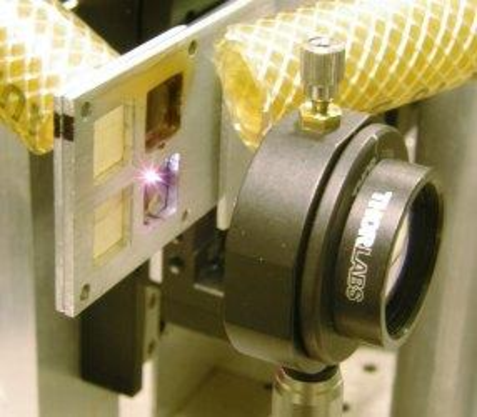
\includegraphics[height=5cm]{img/technology/sieve2_drilling_m.pdf}
\textbf{b)}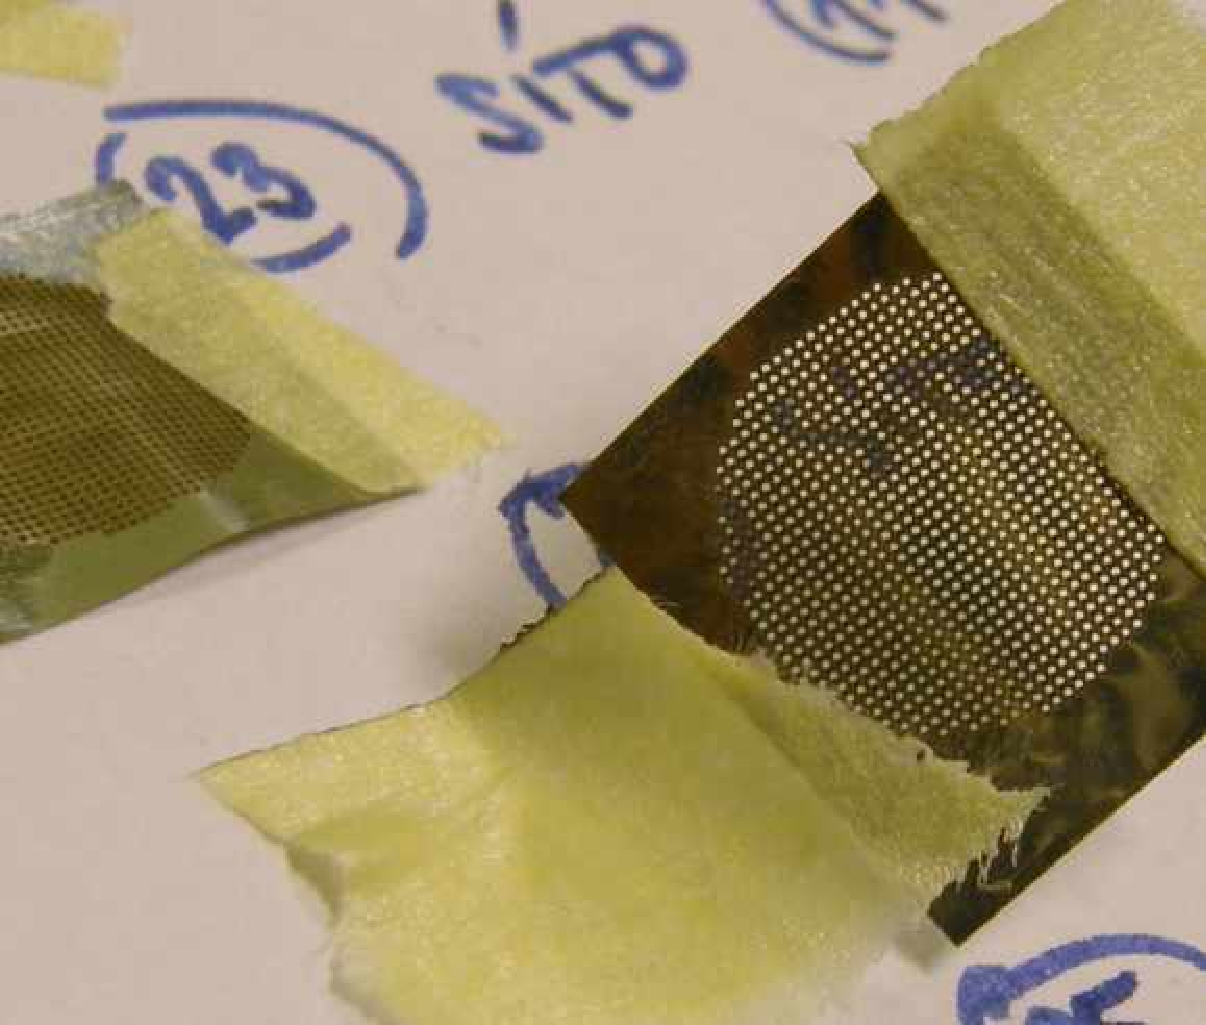
\includegraphics[height=5cm]{img/technology/steel_sieve_on_paper.pdf}
\end{figure}

To achieve the required precision of sieving, we fabricated the sieves by femtosecond laser drilling of 20 $\upmu$m thick stainless steel sheets (Fig. \ref{fg_microfab}). 
%These sieves then were employed in a device that subjected the microsphere sample to acoustic vibrations, improving the speed of the demanding sieving process to acceptable level (Fig. \ref{fg_microfab}b,c).
\add{ TODO}


\add{Owing to the homogeneous broadening of the resonator resonance, caused by intrinsic losses of TiO$_{2}$, further sieving appears to lack any purpose. Not only this project broadens the numerous group of technically successful research projects pointed in utterly wrong direction, it also classifies into the lamentable subgroup of effort that could be entirely avoided if open and honest scientific discussion took place about the inherent problems. In this case, particularly, in all related papers it should be openly stated, that the dielectric losses of TiO2 prevent building any applicable volume metamaterial, no matter how accurately the resonators are prepared.}

